%
% File:     chapter-systemmodel.tex
% Author:   awl8049
% Revision: $Revision: 2.2 $
%
\chapter{System Modeling}
\label{chp:modelstruct}
In order to develop a deterministic continuous energy consumption model
based on computational load of the system, we consider $E_{dc}$, the
total DC power input to the system, at the output of the power supply.
Most servers operate on the AC input, with efficiency of power
conversion from AC to DC equal to 72 - 80\% (depending on the system
load~\cite{ton2008}) and with the DC output delivered in the domains of
+/-12V, +/-5V, and +/-3.3V \cite{SSI2004}.  Typically, two 12 Vdc lines
supply power to the processor's hard drive(s) and cooling fans in the
system.  The 5 Vdc and 3.3 Vdc lines are dedicated to supplying power to
the support chips and peripherals on the board.

Energy delivered to a server system, $E_{dc} = E_{system}$, can be
expressed as a sum of energy consumed by constituent sub-systems in the
server.  Generally, there are five sources of energy consumption in a
server system:
\begin{description}
\item{$E_{proc}$:} Energy consumed in the processor due to computation,
\item{$E_{mem}$:} Energy consumed by DRAM chips,
\item{$E_{hdd}$:} Energy consumed by the hard disk drive(s),
\item{$E_{board}$:} Energy consumed by peripherals in support of board the
  operations, including all devices in multiple voltage domains across the board
  (like chip-set chips, voltage regulators, bus control chips, connectors, interface devices, etc.),
\item{$E_{em}$:} Energy consumed by all electrical and electromechanical
  components in the server, including fans and other support components.
\end{description}

Total energy consumed by the system with a given computational workload
can be expressed as:
\begin{equation}
\label{eq:linmodel}
E_{system}= E_{proc} + E_{mem} + E_{hdd}+ E_{board} +  E_{em}.
\end{equation}
Each of the above terms is explored in turn by following an energy
conservation principle.  In order to get a true measure of the
computational load on the system, our approach snoops on bus
transactions per unit time (indicated by PeC readings), measures the
temperature changes (in die and ambient sensor readings), and records
the speeds of cooling fans, in the course of job execution.  The use of
those PeCs and metric readings fits well to NUMA-based multi-core
processors. 
\begin{figure*}[tp]
  \begin{minipage}{0.5\linewidth}
  \centering
     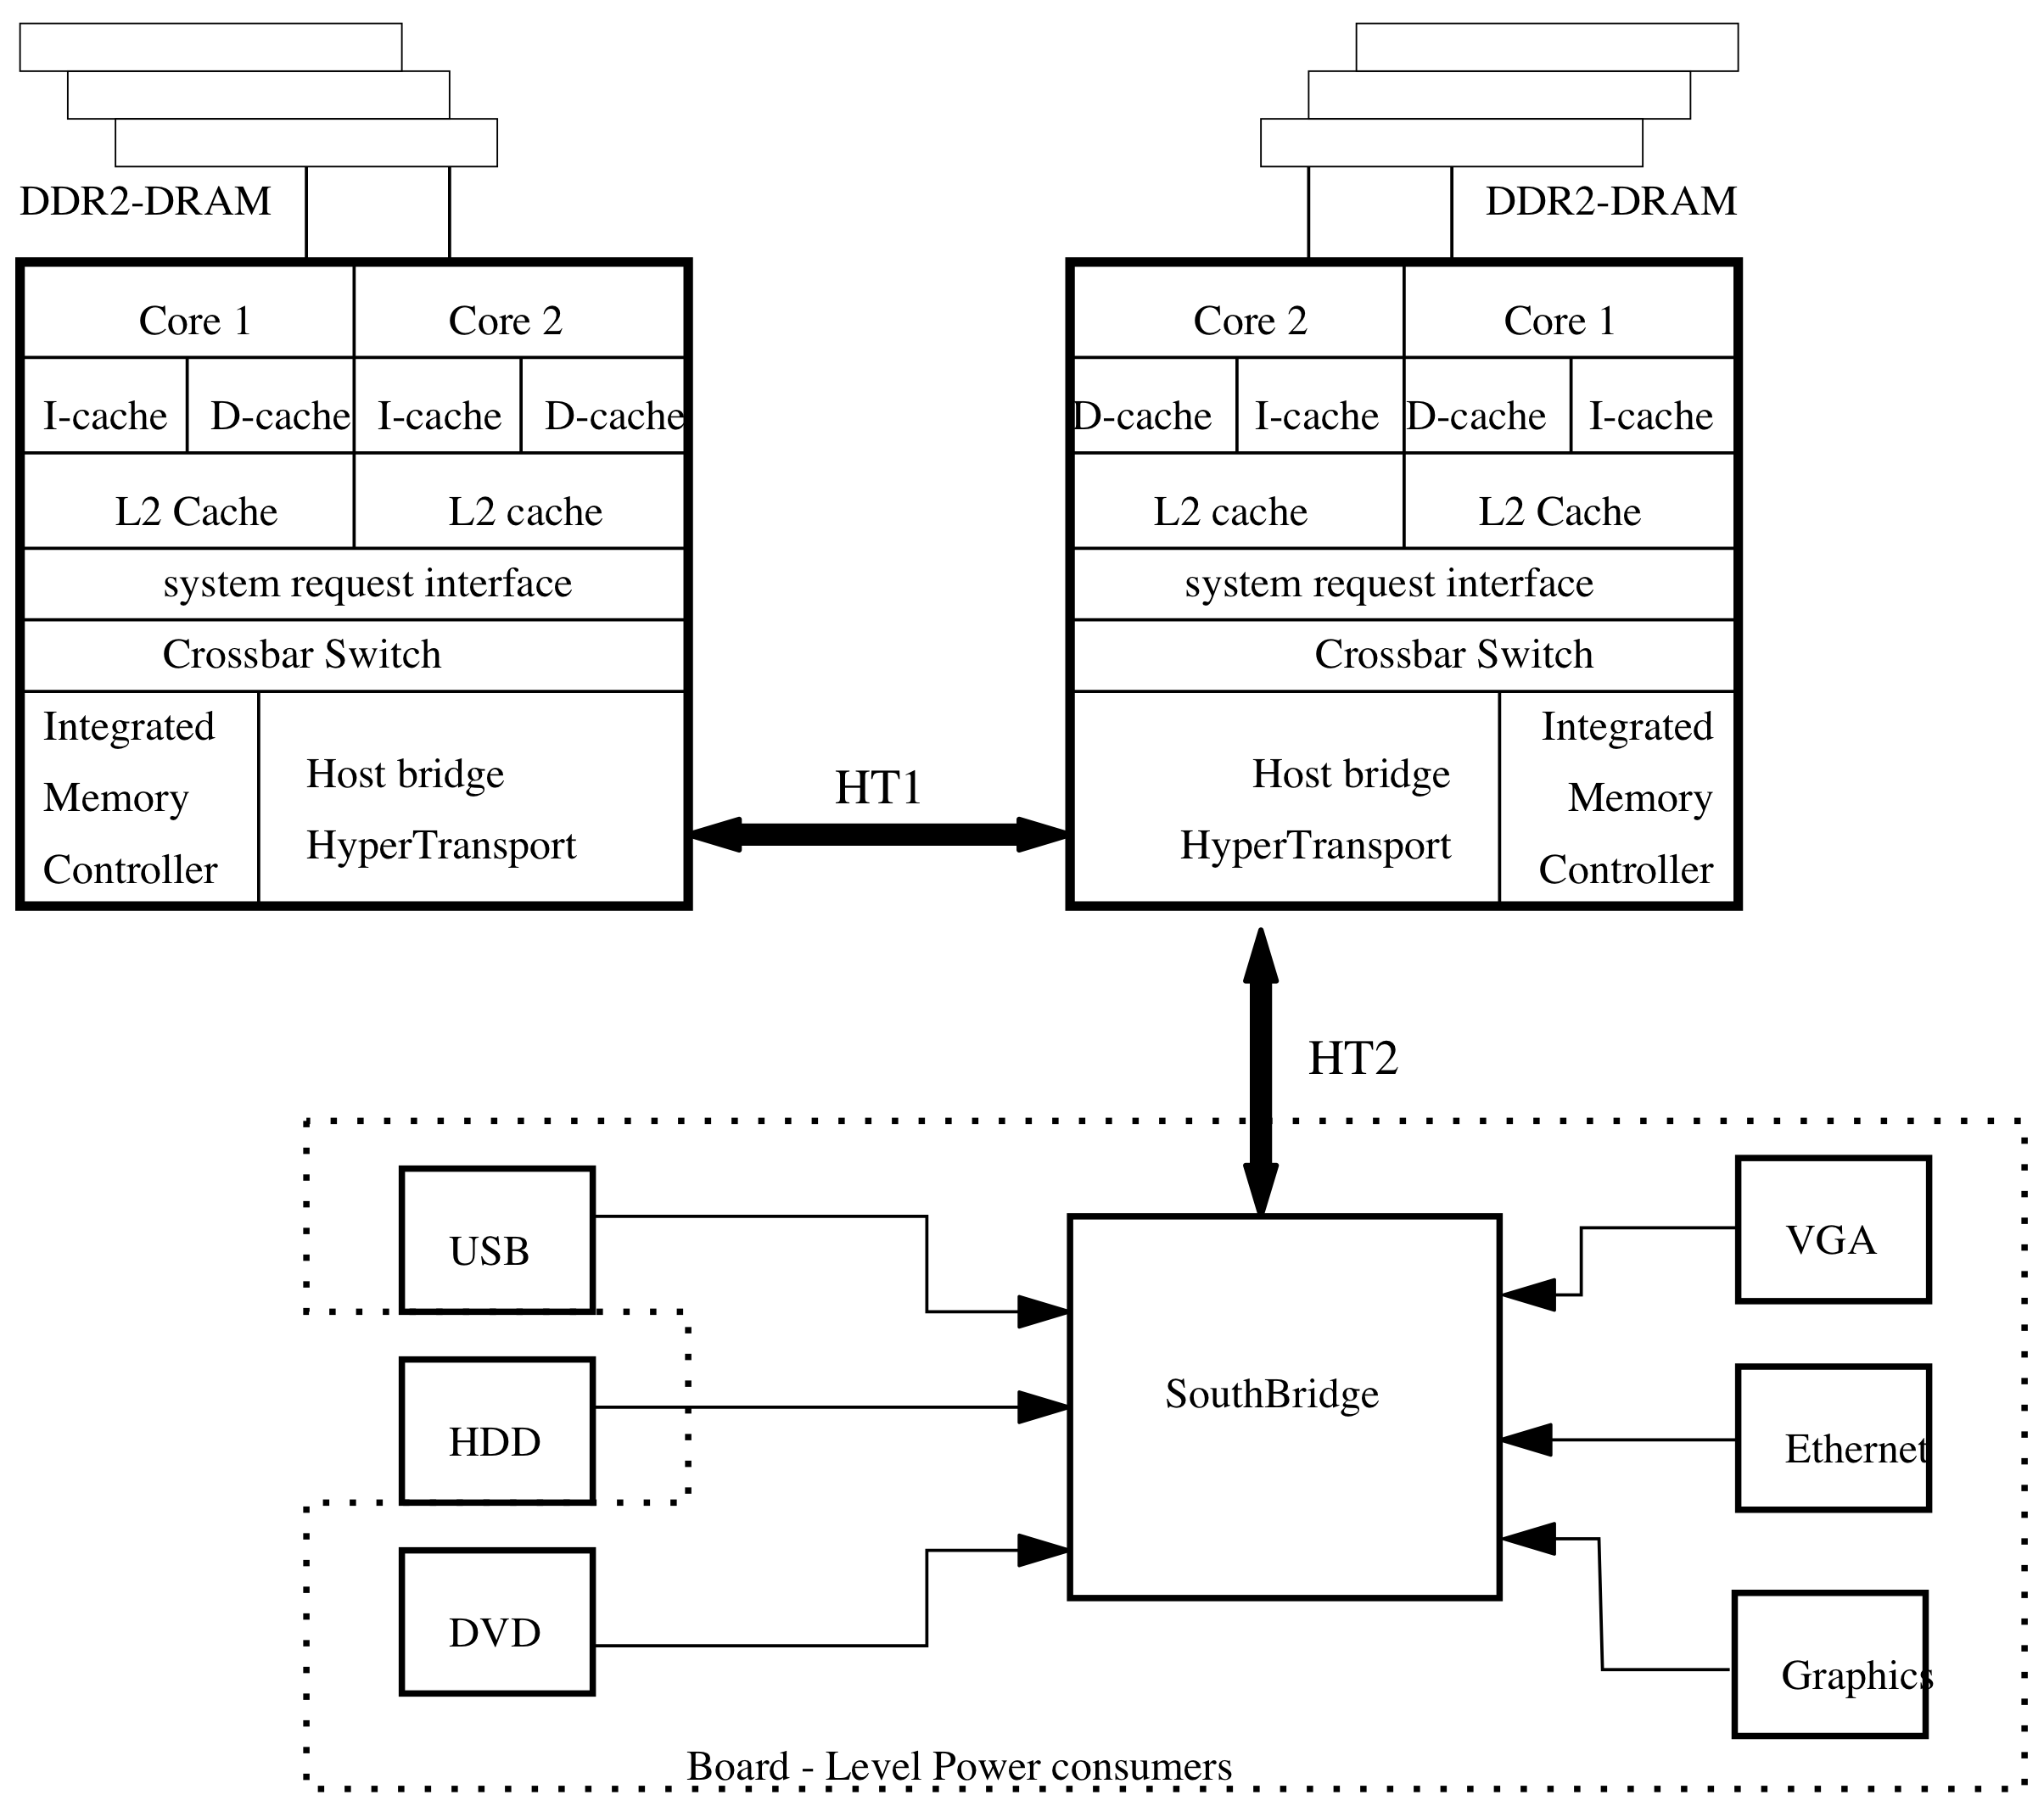
\includegraphics[scale=0.3]{x2200sys}
     \caption{AMD Opteron architecture.}
     \label{fig:amdarch}
  \end{minipage}\hspace{0.1cm}
  \begin{minipage}{0.5\linewidth}
  \centering
     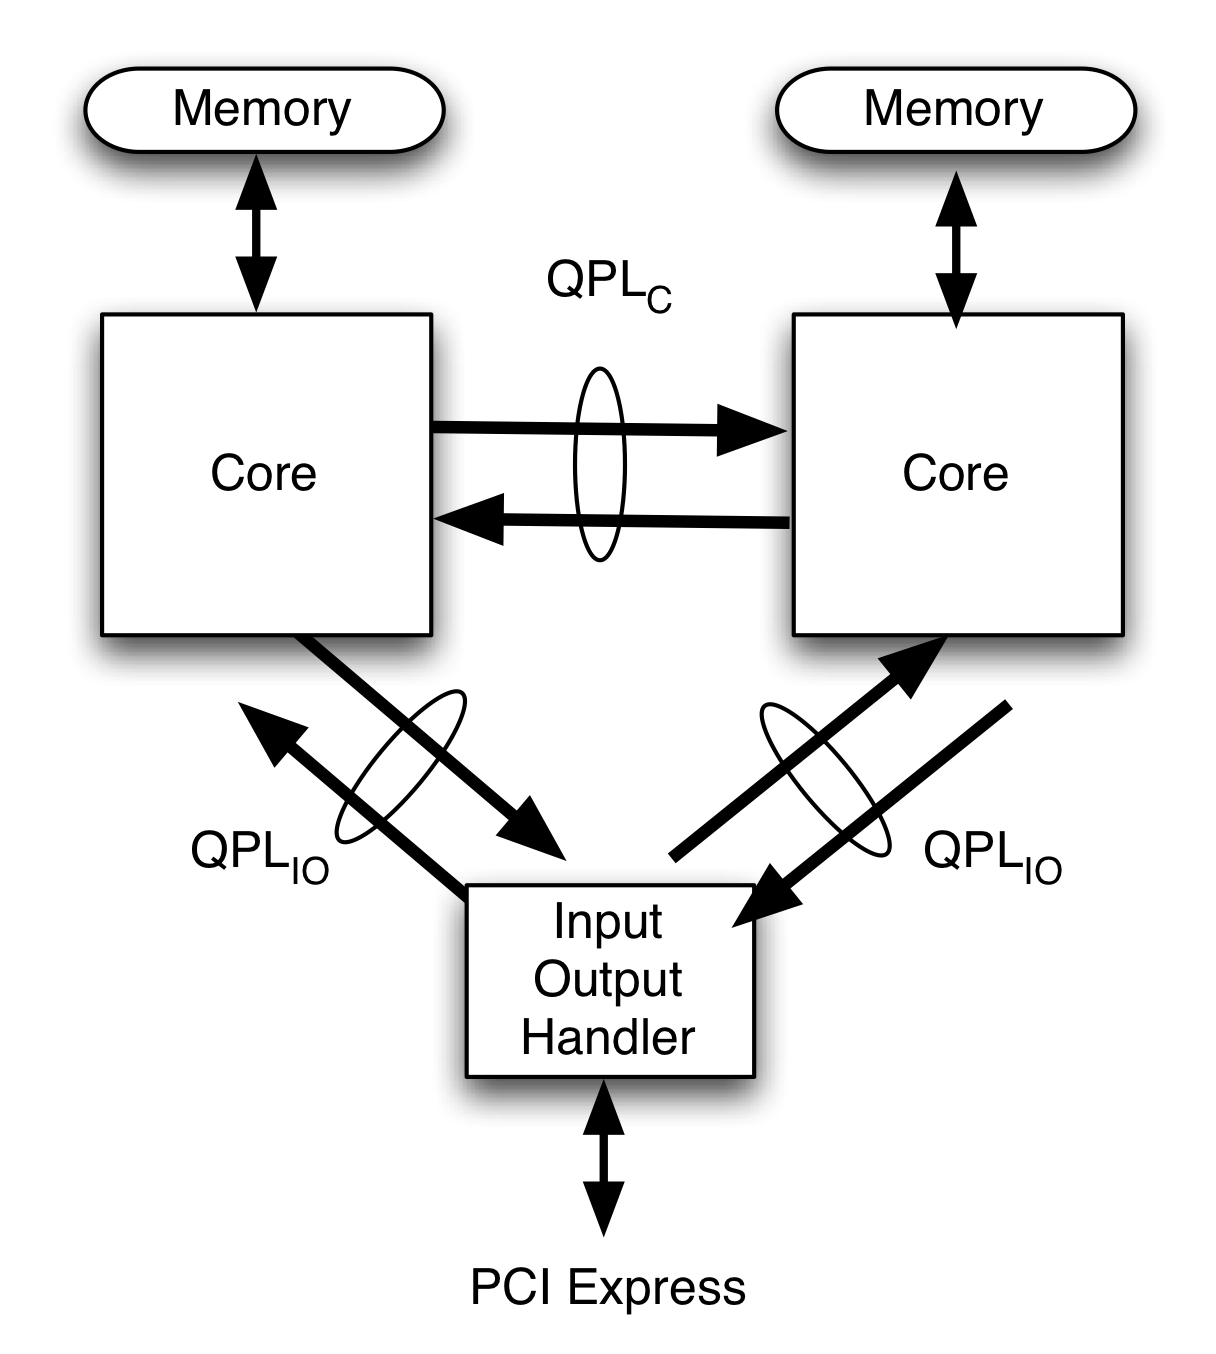
\includegraphics[width=1.0\textwidth,scale=0.5]{intelnehalem}
     \caption{Intel Xeon (Nehalem) architecture.}
     \label{fig:intarch}
  \end{minipage}
\end{figure*}
\section{Processor energy consumption}
\label{sec:procmodel}
Consider the AMD Operton architecture and the Intel Nehalem
architecture, as depicted in \figurenames~\ref{fig:amdarch} and
\ref{fig:intarch}.  The former is a NUMA-based processor
(\figurename~\ref{fig:amdarch}), with Northbridge functionality
incorporated in the processor core and each core responsible for local
access to the memory connected to that Northbridge logic (shown in
\figurename~\ref{fig:amdarch} as ``Integrated Memory Controller'').
Processor cores on a single die are connected via a crossbar to the
HyperTransport bus (i.e., HT1) between processors.  A coherent bus
protocol is used to ensure memory consistency between processor cores on
each die.  In addition, the master processor in the system is connected
via a second HyperTransport bus (i.e., HT2) to the Southbridge device
that manages connections to the outside world.  A similar structure
exists in the Intel Xeon Nehalem architecture.  Unlike the AMD Operton,
each Nehalem processor is connected to an Input-Output handler, which
provides the Southbridge with connecting functions for off-chip resources.

It is observed that work done by any of the processors, as the heart of
energy consumption in a server system, can be quantified in terms of bus
transactions in and out of the processors.  Traffic on the external
buses provides a measure of how much data is processed by the processor.
In the case of the NUMA architecture, this quantity can be measured by
determining the amount of data transmitted over interconnect between
processor cores (HyperTransport for AMD processors, QPI links for recent
Intel processors). Our energy consumption model aims to treat each
processor as a black box, whose energy consumption is a function of its
work load (as manifested by core die temperatures measured at the system
level by \texttt{ipmitool} through sensors on the path of the outgoing
airflow from the processor).  In practice, when estimating processor
power consumption based on PeCs (performance counters), there are only a
limited number of PeCs for tools, like \texttt{cpustat}, to track
simultaneously.

For the AMD dual-core Operton architecture (shown in
\figurename~\ref{fig:amdarch}), traffic on the HT buses is viewed as a
representative of the processor workload, reflecting the amount of data
being processed by a processor (i.e., its involved cores).  The HT2 bus
is non-coherent and connects one of the two processors to the
Southbridge (whereas the Northbridge is included on the Opteron
processor die).  Thus, traffic on the HT2 bus reveals hard-disk and
network transactions.  This model scales by considering the effect of
network traffic and disk I/O transactions.  HT1 is a coherent bus
between the two SMP processors and, as such, PeCs on HT1 provide
accurate estimation on the processing load of cores executing jobs.
Per-core die temperature readings are directly affected by the number of
transactions over the HT1 bus.  A similar observation holds for the QPL
links present in the Intel Nehalem architecture, with traffic between
its two cores reflected by transactions on QuickPath Links between the
cores, denoted by $QPL_C$ (see \figurename~\ref{fig:intarch}).

Therefore, total processor power consumption at time $t$, $P_{proc}(t)$,
is related to processor temperature readings and the estimated amount of
data being processed at the time, and it can be expressed as a function
of three metrics: die temperature readings for processors 0 and 1, and
the number of bus transactions (i.e., traffic over HT1 for the AMD
server and over $QPL_C$ for the Intel server).  We have processor energy
consumption between times $t_{1}$ and $t_{2}$ as follows:
\begin{equation}
  \label{eq:procpwr2}
  E_{proc}=\displaystyle\int_{t_{1}}^{t_{2}}\left( {P_{proc}(t)} \right)dt.
\end{equation}
\section{DRAM energy consumption}
\label{sec:dram}
Energy consumed by the DRAM banks is directly related to the number of
DRAM read/write operations involved during the time interval of
interest, and the number is reflected by (1) the last-level cache misses
for all $N$ constituent cores ($CM_{i}(t)$, $i$ = 1, 2, ..., $N$) in
the server when executing jobs and (2) the data amount due to disk
accesses for OS support (like page tables, checkpoints, virtual
environments) and due to performance improvement for peripheral devices
(like buffered data for disks and optical devices, spooled printer
pages).  The data amount in (2) above, named $DB(t)$, is reflected by
traffic over $HT_{2}$ (or QuickPath links between the two cores and the
Input/Output handler, denoted by $QPL_{IO}$) for the AMD Opteron server
(or the Intel Xeon server), as demonstrated in
\figurename~\ref{fig:amdarch} (or \figurename~\ref{fig:intarch}).
This is because network traffic does not exist in either testing server,
which comprises only a single chip.  Additional energy contributors
include activation power and DRAM background power (due to leaking
currents), represented by $P_{ab}$.  As stated earlier
\cite{Micron2007}, DRAM activation power and background power can be
obtained from the DRAM documentation, and they together amount to 493 mW
for one DRAM module in our AMD Opteron server.  Consumed energy over the
time interval between $t_{1}$ and $t_{2}$ can be expressed by
\begin{equation*}
  \label{eq:dram}
  E_{mem}=\displaystyle\int_{t_{1}}^{t_{2}}\left( (\sum_{i=1}^{N}CM_{i}(t)+DB(t))\times
    P_{DR}+P_{ab}\right)dt,
\end{equation*} 
where $P_{DR}$ refers to DRAM read/write power per unit data.
\begin{table}[tp]
\caption{Hitachi HDT725025VLA360 disk power parameters}
\centering
\begin{tabular}{ l l }
\hline
\textbf{Parameter} & \textbf{Value} \\
\hline
  Interface & Serial ATA\\
  Capacity & 250 GB\\
  Rotational speed & 7200 rpm  \\
  Power & \\
  ~~Spin up& 5.25 W (max)\\
  ~~Random read, write & 9.4 W (typical)\\
  ~~Silent read, write & 7 W (typical)\\
  ~~Idle & 5 W (typical)  \\
  ~~Low RPM idle & 2.3 W (typical for 4500 RPM)\\
  ~~Standby & 0.8 W (typical)\\
  ~~Sleep & 0.6 W (typical)\\
\hline
\end{tabular}
\label{tab:hddparam}
\end{table}
\section{Hard disk energy consumption}
\label{sec:networkengery}
Energy consumed by the hard disk(s) is approximated by using a
combination of relevant PeCs and drive ratings. Building a full-system
model of disk drive energy consumption is complicated by the distance
(from the processor) and the high latency of the disk drive.  Two
earlier modeling approaches exist, with one analyzing drive performance
and capacity based on the physical characteristics of the
drive~\cite{Gurumurthi2005} and the other utilizing PeCs (which measure
DMA accesses on the memory bus, uncacheable accesses, and interrupts) to
estimate the value of $E_{hdd}$~\cite{Bircher2011}.

By contrast, our disk model is interested in the amount of information
being transferred back and forth to the device.  So, it is possible to
calculate this value using information collected by the operating system
and physical characteristics of the disk drive. Both our test servers
use the Hitachi's SATA hard disk (whose specification and relevant power
consumption figures are listed in Table ~\ref{tab:hddparam}).  Based on
the physical, electrical, and electromechanical parameters of a hard
disk, one can construct its detailed power consumption model.  However,
a cruder but simpler model can be obtained from the typical power
consumption data of hard disks and pertinent PeCs, including (1) the
number of reads and writes per second to the disk and (2) the amount of
data (in kilobytes) read from and written to the disk.  Those PeCs can
be measured by the tool of \texttt{iostat}, arriving at approximate disk
power consumption, $E_{hdd}$, as:
\begin{align*}
\label{eq:hddpwr1}
E_{hdd} = &P_{spin-up}\times T_{su}+  P_{read}\sum N_r\times T_r \nonumber\\
        &+ P_{write}\sum N_w\times T_w+ \sum P_{idle}\times T_{id}
\end{align*}
where $P_{spin-up}$ is the power required to spin-up the disk from 0 to
full rotation, and $T_{su}$ is the time required to achieve spin up,
typically about 10 sec.  $P_{read}$ (or $P_{write}$) is the power
consumed per kilobyte of data read from (or written to) the disk,
whereas $N_r$ (or $N_w$) is the number of kilobytes of data reads (or
data writes) in time-slice $T_r$ from (or to) the disk.  The Hitachi
disk achieves read operations at 1.5 Gbits/s, when consuming 530 mA
current at +5V, thereby exhibiting approximately $13.3 \mu W$/Kbyte.
Similarly, it is found to consume $6.67 \mu W$/Kbyte for write
operations.  The numbers of $N_r$ and $N_w$ can be obtained using
\texttt{iostat} according to the chosen time slice.

There are two idle states for the disk: idle and unloaded idle (when
disk read/write heads are unloaded).  The time to go from the unloaded
idle state to the idle state is usually less than 1 second (smaller than
the resolution of \texttt{iostat}).  Thus, a history match count in the
\texttt{iostat} statistics with zero reads and writes signifies the
periods in which the disk is idle, permitting us to compute idle energy
consumption accordingly.  \texttt{iostat} readings for the durations of
switching to different disk power states may be obtained with a more
in-depth analysis, which is not consider in this work.

\section{Board energy consumption}
\label{sec:board}
The quantity of $E_{board}$ represents energy consumption caused by the
support chipsets, control logic, buses, signal links, etc., and it
usually falls into the 3.3V and 5V power domains.  Exhibiting little
variation, $E_{board}$ can be difficult to measure, as chipset power is
drawn from multiple domains.  Hence, earlier
models~\cite{Kansal2010,Bircher2011} treated $E_{board}$ as a
constant. In our case, however, this value is obtained using current
probe-based measurements.  The results are measured over an interval of
interest, $t_{interval}$ and exclude the effects of processor, disks,
fans, and optical devices.  Note that introducing the current sensors
(possibly taking up to 28 for a server ~\cite{SSI2004}) to the power
lines on the board will provide instantaneous current readings for use
in $E_{board}$.

Aggregated power consumption effects on the board may be captured using
ambient temperature readings on the board.  Such readings can be
obtained using system management tools commonly found in server
environments (such as IPMI), and they are included in the set of our PeCs
for energy consumption estimation.

\section{Electromechanical energy consumption}
\label{sec:electrical}
A server always involves electromechanical energy consumption, $E_{em}$,
which is mainly due to the electromechanical functions related to system
cooling.  Multiple fans often exist in a server for cooling.  Power
drawn by the $i^{th}$ fan at time $t$ can be given by the following
equation:
\begin{equation}
\label{eq:fanp}
P_{fan}^{i}(t) = P_{base} \times \left(\frac{RPM_{fan}^{i}(t)}{RPM_{base}}\right)^3
\end{equation} 
where $P_{base}$ defines the base power consumption of the unloaded system
when running only the base operating system and no application workload.
The $P_{base}$ value is obtained experimentally by measuring the current drawn
on the +12V and +5V lines, using a current probe and an oscilloscope.
There is a current surge at system start, which is neglected.
Under nominal conditions, the +12V line draws approximately 2.2A
to power both blower fans in the AMD testing server. Total electromechanical energy consumption over a given task execution
period of $T_{p}$ equals:
\begin{equation*}
\label{eq:elect}
E_{em} =  \int^{T_{p}}_0 \left(\sum_{i=1}^NP_{fan}^{i}(t)\right)dt.
\end{equation*} 

\section{Extending the model for thermal behavior}
\label{sec:extend-model-therm}
An application is composed of $p$ execution threads, each associated with a
data set sized $d_{i}$, for $1\leq i \leq p$, in a processor. The total
data associated with $A$ is the sum of the data associated with its
component threads:
\begin{equation}
\label{eq:totaldata} D_{A}=\displaystyle\sum_{i=1}^{p}{d_i}.
\end{equation} 
We assume that the activities take place (1) in a staging area,
which contains both main and virtual memory operating space,
and (2) in the processor with its cores and their associated caches.
The execution time measurement includes 
computation time and the time to move application data from the
staging area (on peripherals off the chip like DRAM and HDD) to a
computation or operation area (on the chip, such as the caches and the cores).

Each application $A$ with the problem size of $D_{A}$ involves workload
$W(\tau_{i},d_{i},t_{i})$, for $1 \leq i \leq p$, comprising two
components: (1) a count of the operations performed by the computational
core, and (2) the count of communication operations required for
transferring data, instructions, and data coherency and book-keeping
functionality traffic.  They are measured in terms of the number of
bytes operated upon or transferred over, during the course of completing
those instructions retired by the logical core for each thread $p$.
Thus, energy consumed by executing application $A$ with data set $D_{A}$
can be expressed as:
\begin{equation}
\label{eq:eworkload} 
E_{A}(A,D_{A},t) = \displaystyle \sum_{i=1}^{p}W(\tau_{i},d_{i},t_{i})
\end{equation}
for $1\leq i \leq p$, where $\tau_{i}$ is an execution thread involved in
application $A$, $d_{i}$ is the corresponding data set for that thread,
and $t_{i}$ is its thread execution time.

In order to relate system energy expenditure (upon application
execution) to corresponding joule heating, we define the term of
``Thermal Equivalent of Application'' (TEA), as the electrical work
converted to heat in running the application, leading to die temperature
change and ambient temperature change of the system.  Hence, the TEA of
application $A$ is expressed by:
\begin{equation}
\label{eq:tea} \Theta(A, D_{A}, T, t) =
\frac{E_{A}(A, D_{A}, t)}{\displaystyle \lim_{T \to T_{th}} J_e(D_{A}, \Psi_{cp}) (T -T_{nominal})},
\end{equation} 
where $T_{th}$ denotes the threshold temperature at which a thermal
emergency event will occur, and $T_{nominal}$ refers to the nominal
temperature as reported by the system when it is in a quiescent state,
i.e., only the operating system is running without any application
execution.  The term $J_{e}$ is the ``electrical equivalent of heat''
for the chip, which reflects the \textit{informational
  entropy} of the system due to processing the data bits
during application execution and to the black body thermal properties of
the chip packaging as well as the cooling mechanisms around the chip, as
defined by the parameter $\Psi_{cp}$.  The value of $\Psi_{cp}$ is an
ambient thermal characterization parameter provided by the hardware
manufacturer to relate temperature to power for cooling
purposes~\cite{Intel2006}.  Thus, TEA is a dimensionless quantity, with
both denominator and numerator expressing work done or energy consumed
in finishing an application.

We combine these metrics into achieved performance per unit energy
consumed by the chip:
\begin{equation}
\label{eq:thermcost} C_{\theta}(A, D_{A}, T, t)=\frac{\Theta (A, D_{A}, t)}{E_{system}(A, D_{A}, t)}
\end{equation}
This normalized quantity indicates the ``cost'' of executing an
application on a given processor, with $E_{A}(A, D_{A}, t)$ obtained
from energy consumption of individual physical components (processor,
DRAM units, HDD, motherboard, and electrical/electromechanism) given by
\equationname~\eqref{eq:linmodel}.

% Following comment block used by GNU-EMACS and AUCTEX packages
% Please do not remove.
%%% Local Variables: 
%%% mode: latex
%%% TeX-master: "dissertation.tex"
%%% TeX-PDF-mode: t
%%% TeX-source-correlate-mode: t
%%% End: 
